\begin{figure}[t]
        \centering
        {
            \begin{tabular}{ccc}
                \hspace{-2mm}
                {
\includegraphics[width=0.19\linewidth]{./img/ablate_nfd/materials/input}}
                {
\includegraphics[width=0.19\linewidth]{./img/ablate_nfd/materials/wo_n}}
                {
\includegraphics[width=0.19\linewidth]{./img/ablate_nfd/materials/w_n}}
                {
\includegraphics[width=0.19\linewidth]{./img/ablate_nfd/materials/wo_a}}
                {
\includegraphics[width=0.19\linewidth]{./img/ablate_nfd/materials/w_a}}
                \\
                \hspace{-2mm}
                \subcaptionbox{\scriptsize Input}{
\includegraphics[width=0.19\linewidth]{./img/ablate_nfd/ficus/input}}
                \subcaptionbox{\scriptsize w/o NFD}{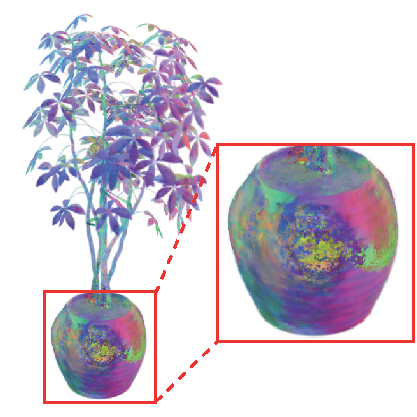
\includegraphics[width=0.19\linewidth]{./img/ablate_nfd/ficus/wo_n}}
                \subcaptionbox{\scriptsize w/ NFD}{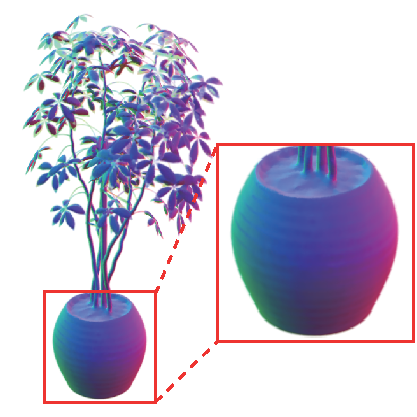
\includegraphics[width=0.19\linewidth]{./img/ablate_nfd/ficus/w_n}}
                \subcaptionbox{\scriptsize w/o NFD}{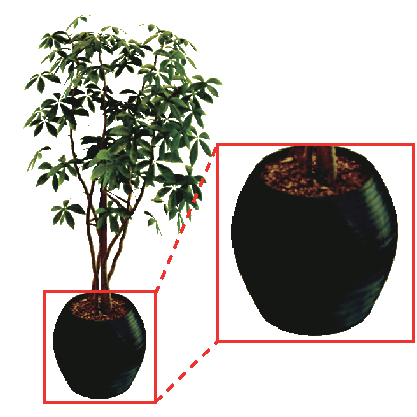
\includegraphics[width=0.19\linewidth]{./img/ablate_nfd/ficus/wo_a}}
                \subcaptionbox{\scriptsize w/ NFD}{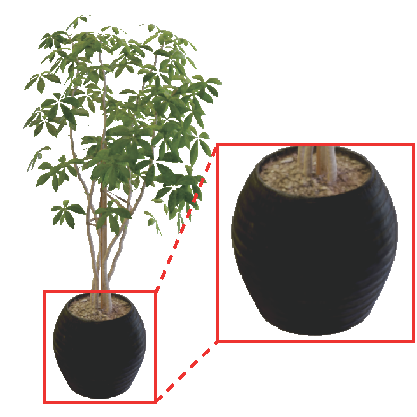
\includegraphics[width=0.19\linewidth]{./img/ablate_nfd/ficus/w_a}}
            \end{tabular}
        }
        \caption{
            Qualitative comparisons between decomposed normals and diffuse albedos with normal field distillation (w/ NFD) and without normal field distillation (w/o NFD). 
        }
        \label{fig:ablate_NFD}
\end{figure}
